\contourlength{1.0pt}
\tikzset{>=latex} % for LaTeX arrow head

\colorlet{xcol}{blue!60!black}
\colorlet{myred}{red!85!black}
\colorlet{myblue}{blue!80!black}
\colorlet{mycyan}{cyan!80!black}
\colorlet{mygreen}{green!70!black}
\colorlet{myorange}{orange!90!black!80}
\colorlet{mypurple}{red!50!blue!90!black!80}
\colorlet{mydarkred}{myred!80!black}
\colorlet{mydarkblue}{myblue!80!black}
\tikzstyle{xline}=[xcol,thick]
\tikzstyle{Tline}=[line width=0.6]
\tikzstyle{width}=[{Latex[length=5,width=3]}-{Latex[length=5,width=3]},thick]
\def\tick#1#2{\draw[thick] (#1)++(#2:0.12) --++ (#2-180:0.24)}
\def\N{100} % number of samples

% HARMONIC OSCILLATOR FORCE




% HARMONIC OSCILLATOR ENERGY
\def\ymax{1.4} % max y axis


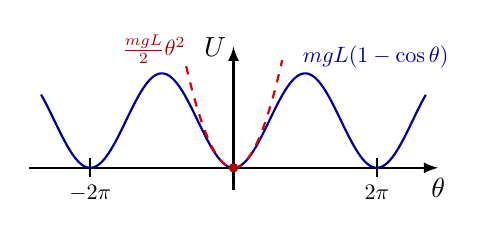
\begin{tikzpicture}
  \def\xmax{2.6} % max x axis
  \message{^^JHarmonic oscillation}
  \def\A{0.6}         % amplitude
  \def\T{(0.7*\xmax)} % period
  \draw[->,thick] (0,-0.2*\ymax) -- (0,1.1*\ymax) node[left=-1] {$U$};
  \draw[->,thick] (-\xmax,0) -- (\xmax,0) node[below] {$\theta$};
  \draw[xline,samples=100+\N,smooth,variable=\x,domain=-0.94*\xmax:0.94*\xmax]
    plot(\x,{\A-\A*cos(360/\T*\x)});
  \draw[xline,myred,dashed,samples=\N,smooth,variable=\x,domain={-0.33*\T}:{0.34*\T}]
    plot(\x,{\A/2*(2*pi*\x/\T)^2});
  \fill[myred!80!black] (0,0) circle(0.06);
  \tick{{\T},0}{90} node[below=0,scale=0.8] {$2\pi$};
  \tick{{-\T},0}{90} node[below=0,scale=0.8] {$-2\pi$};
  \node[mydarkred,above left,scale=0.8] at ({-0.28*\T},2.05*\A) {$\frac{mgL}{2}\theta^2$};
  \node[mydarkblue,above right,scale=0.8] at ({0.43*\T},1.95*\A) {$mgL(1-\cos\theta)$}; %U(\theta)=
\end{tikzpicture}
